\documentclass[buriama8_dp.tex]{subfiles}
\begin{document}

\chapter{Experiments}

All steps in implementation of the solution were verified by experiments. We conducted both simulated experiments and experiments on a real robotic arm.

\section{Benchmark environment}
\label{sec:exp_cpp_env}

We created a benchmark environment representing an obstacle in front of the robot. The environment is represented in a grid \(10 \times 10 \times 5\) cells. We also tested the algorithms in free space, to evaluate if they produce paths reasonable to a human eye.

The environment contains two obstacles, a floor-standing object and an overhang above the object, with enough space for the robot to pass through. A single plane extracted from the full 3D environment is used as the 2D benchmark for the coverage algorithm. The planar environment is illustrated in Figure~\ref{fig:2d_env}.

\begin{figure}[htp]
  \centering
  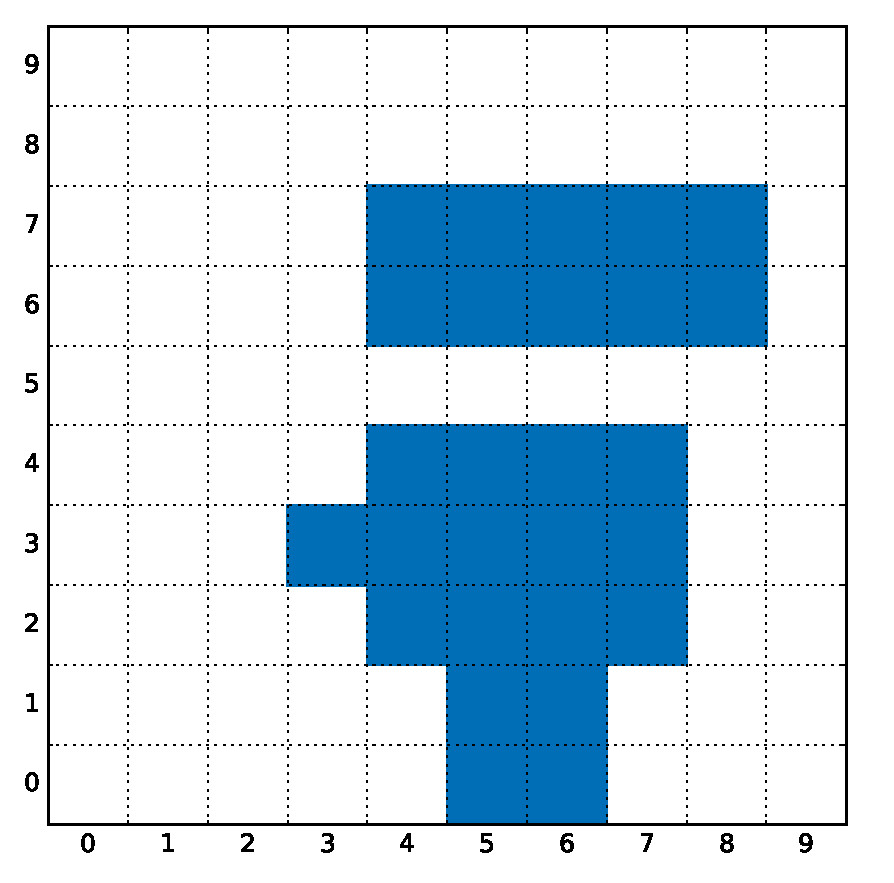
\includegraphics[width=7cm]{2d_coverage_env.pdf}
  \caption[2D benchmark environment]{The 2D benchmark environment for CPP algorithms. The environment is depicted as a vertical slice as seen by the robot; the \uvz{floor} is at the bottom}
  \label{fig:2d_env}
\end{figure}

In simulating coverage algorithms, we ignore the arm collision checking with previously discovered obstales. This is accounted for when we simulate the whole arm.

\section{Simulated coverage algorithms}
\label{sec:exp_sim_coverage}

To test the performance of CPP algorithms we implemented, we peformed experiments to determine how well the methods perform in unknown environments in both 2 and 3 dimensions. Each of the algorithms was run in \REV{an} empty 2D environment to test it in the simplest setting, followed by a run in the benchmark environment described in Section~\ref{sec:exp_cpp_env} Because of the generalization scheme used to adapt the algorithm to explore 3D space, 2D environment is represented in 3D as a grid with only one depth layer.

\subsection{Two dimensions}
\label{subsec:2d_sim}

Running the compact space heuristic algorithm in the 2D environment, we obtained paths depicted in Figure~\ref{fig:heur_2d_coverage}.

\begin{figure}[ht]
  \centering
  \begin{subfigure}[t]{0.49\textwidth}
    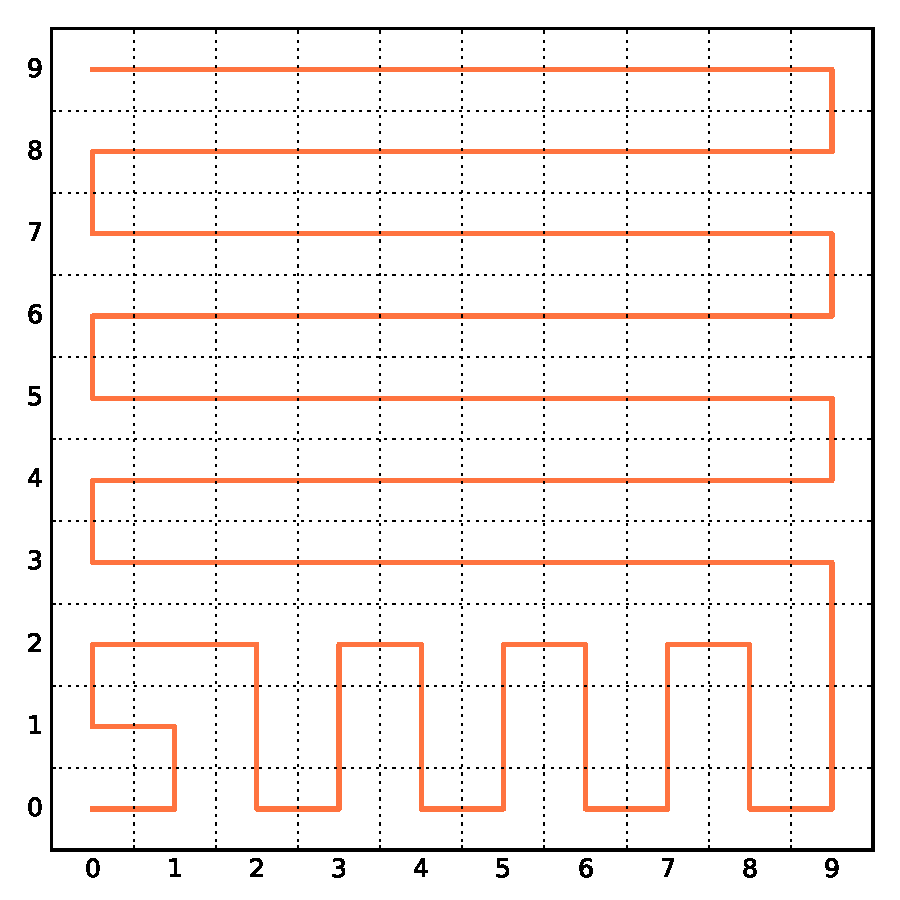
\includegraphics[width=\textwidth]{2d_coverage_heur_empty.pdf}
    \caption{}
    \label{fig:heur_2d_empty}
  \end{subfigure}
  \begin{subfigure}[t]{0.49\textwidth}
    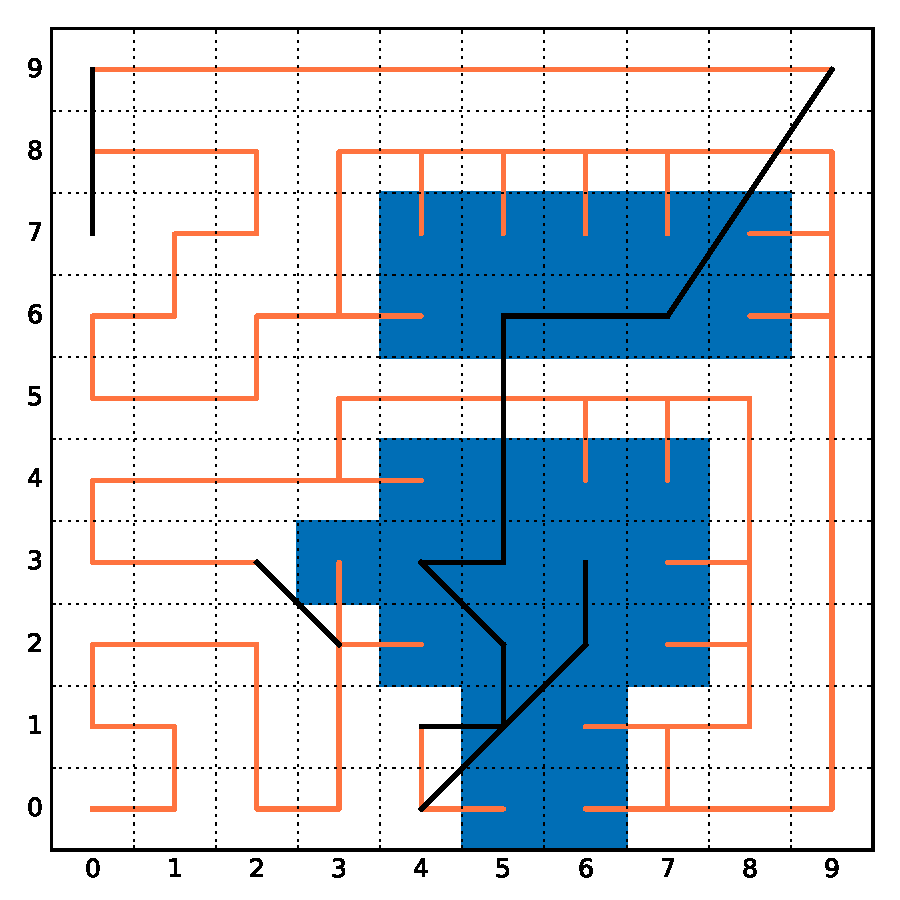
\includegraphics[width=\textwidth]{2d_coverage_heur.pdf}
    \caption{}
    \label{fig:heur_2d_env}
  \end{subfigure}
  
  \caption[Coverage path -- compact space heuristic in 2D]{Coverage path generated by them compact space heuristic in an empty (a) and in the benchmark environment (b). The path starts at \([0,0]\) and is depicted in orange, with transitions to nearest unexplored field depicted in black. The path plot is perturbed by a small amount to let the reader follow it more easily}
  \label{fig:heur_2d_coverage}
\end{figure}

The results in empty space are reasonable. The generated path closely resembles the boustrophedon pattern used in human-designed algorithms. The already explored space is kept compact, as was the aim of the heuristic. The length of the generated path is 9.9\,m, which is the optimal value since no cell was explored twice. This is allowed by the even size of the environment; in case of odd environment width, the lower zig-zag terminates in the lower-right corner and the robot then has to return back to the yet unexplored portion of the environment, travelling through the already known fields again.

In the benchmark environment, we can see that the path starts the same as in the empty environment. When the obstacle is encountered, we can indentify the algorithm following the other incentive it has -- exploring space near known obstacles. This leads to obstacle-circling, after which the obstacle limits are quickly determined. The length of the path is 1.25\,m. \TODO{elaborate}

\subsection{Three dimensions}
\label{subsec:3d_sim}

The results of running the coverage algorithm are shown in Figure~\ref{fig:heur_3d_coverage}.

\begin{figure}[ht]
  \centering
  \begin{subfigure}[t]{0.48\textwidth}
    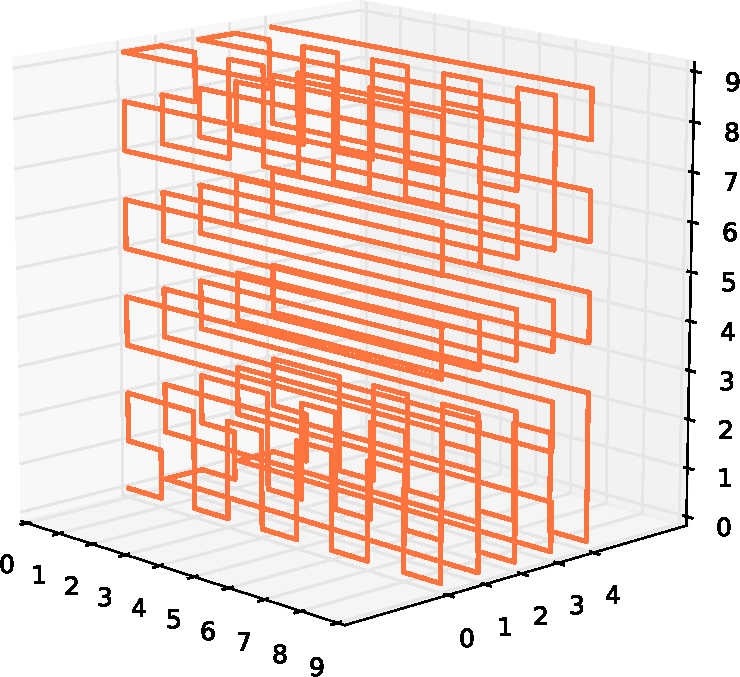
\includegraphics[width=\textwidth]{3d_coverage_heur_empty-cropped.pdf}
    \caption{}
    \label{fig:heur_3d_empty}
  \end{subfigure}
  \;
  \begin{subfigure}[t]{0.48\textwidth}
    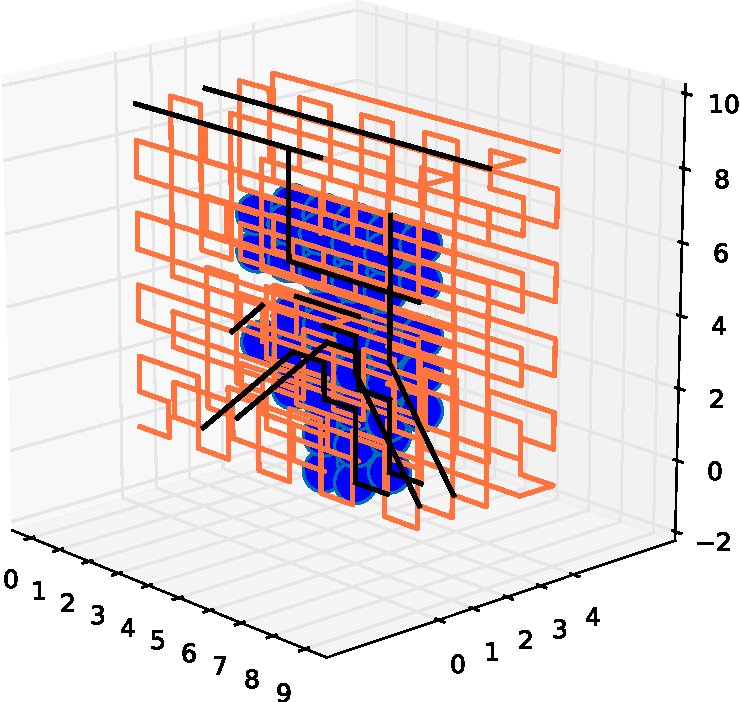
\includegraphics[width=\textwidth]{3d_coverage_heur-cropped.pdf}
    \caption{}
    \label{fig:heur_3d_env}
  \end{subfigure}
  
  \caption[Coverage path -- compact space heuristic in 3D]{The coverage path generated in 3D in (a) empty space and (b) benchmark environment. The obstacles are represented by spheres at the given point}
  \label{fig:heur_3d_coverage}
\end{figure}

Expectedly, the algorithm runs in 3D space as well as in two dimensions. In both cases, we can observe the layers in which the environment has been explored. In the empty environment, the algorithm starts and ends on opposite sides, and thus the layers are identical, only mirrored. The found path is again optimal with length of 49.9\,m.

When obstacles are present, the coverage path is different in each layer partly because of the varying obstacles, partly because of different entry points, as one layer starts precisely where the other has ended. The path is 56.3\,m long.


\section{Simulated arm experiments}
\label{sec:exp_sim_arm}

\subsection{Moving the arm}
\label{subsec:exp_move}

In Sections \ref{subsec:motion_planning} and \ref{subsec:no_plan}, we mention two ways of driving the robot: motion planning and Jacobian transformation. Both have their advantages and disadvantages. We tested them by running the algorithm with each as the robot driving function. We used only the simulated arm ar first to protect the hardware from unfortunate accidents.

We let the simulated arm explore empty space. We evaluated the failures of the movement, such as getting stuck, and the smoothness, precision and optimality of the overall path.

The motion planning method is very reliable in always reaching the desired target pose, and reaching it precisely, when performing a step in the algorithm. In the test run, all the steps were carried out successfuly. The planning took in the order of hundreds of milliseconds for each step. Even when using the TRAC-IK solver, sometimes a joint configuration  very different from the current one was found as the IK solution by the solver. The planner then had no other option than to plan a more complicated path, perhaps rotating the first joint \(180\degr\).

The Jacobian method is extremely fast. The pause at each step is only a few milliseconds, the arm seemingly does not stop at all. We tested the control algorithm by driving the arm across its workspace along the \m x axis. The arm followed the given trajectory with tolerance of 2\,mm. To further improve the here completely satisfactory result, we turned on the error correcting term described in Section~\ref{subsec:impl_drv_jacob}. The precision then got near perfect, with error of at most 0.4\,mm. The errors are depicted in Figure~\ref{fig:err_jac_real}. 

\begin{figure}[ht]
  \centering
  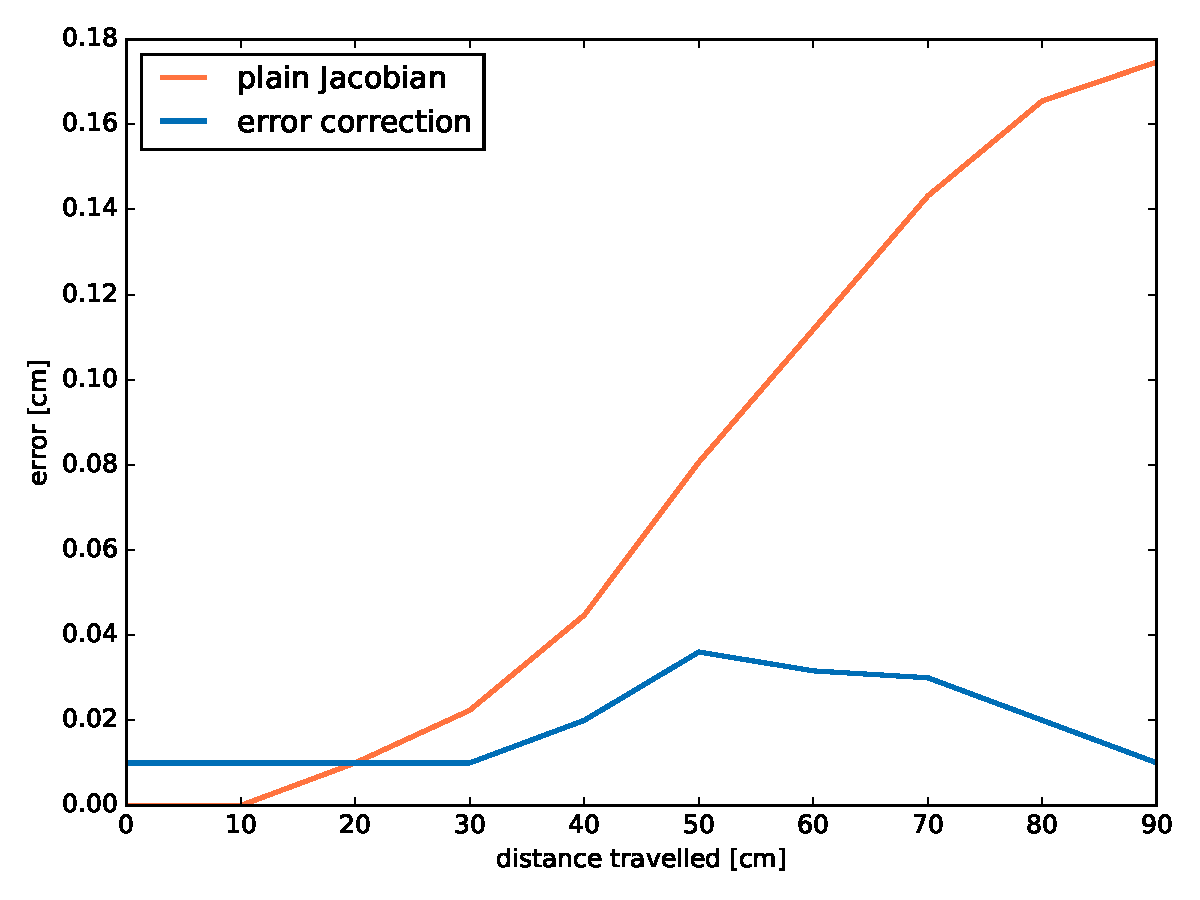
\includegraphics[width=7cm]{jacob_error_sim.pdf}
  \caption{Position error during simulated test drive}
  \label{fig:err_jac_sim}
\end{figure}

The error is probably caused by the numerical error attained in integrating the speeds in discrete steps in the control loop.

In some cases, mostly directly in front of the arm base, a near singularity is reached. Such configuration appears in the test trajectory at 45\,cm, where the end effector passed in front of the base. While we attempt to solve things by slowing the arm down (see the implentation details in Section~\ref{subsec:impl_drv_jacob}), in some configurations, we get so close to the exact singular configurations that no slow-down helps. The driving algorithm identifies such situations and reports failure to higher layers.

The final combined solution described in Section~\ref{subsec:impl_drv} proved to combine the best properties of both the methods. The fallback to planning is used exactly when neccessary. In some cases, however, the Jacobian motion gets the arm stuck in an unexplored collision box because of a slow collision check. Then, even planning fails to move to explore that cell and it is misclassified as unreachable. This results in false positive obstacles identified in the environment.

\subsection{Exploring 3D environment}
\label{subsec:sim_arm_cover}

We tested the final coverage algorithm first in the simulator. We ran it first in empty environment, then in the benchmark environment. The benchmark environment was simulated by publishing false force readings when the arm explored an occupied point.




\section{Real arm experiments}
\label{sec:exp_real_arm}

\subsection{Moving the arm}
\label{subsec:label}

We aimed to confirm the results of movement simulation on the real hardware. Motion planning exhibited the same bahavior as in the simulation. It worked reliably, but in some seemingly random cases, a very complicated plan was generated. These complicated motion plans threaten both the spectators and the cable linking the sensing tool to the host computer.

When we repeated the Jacobian control test we used with the simulated arm, we discovered that the real arm deviates from the intended trajectory significantly. After following the same trajectory, the arm deviated 6\,cm in \m y and 4\,cm in \m z direction. In the end, we had to cerrect the arm considerably in both location and orientation. We assume the error was given by our negelction of the arm dynamics, which we implement by assuming the given joint velocity can be reached immediately by the arm.

This high error gave us the incentive to implement the regulator that would correct the errors. The results were excellent, with maximum error along the path 2\,cm and final error  The errors are depicted in Figure~\ref{fig:err_jac_real}. 

\begin{figure}[ht]
  \centering
  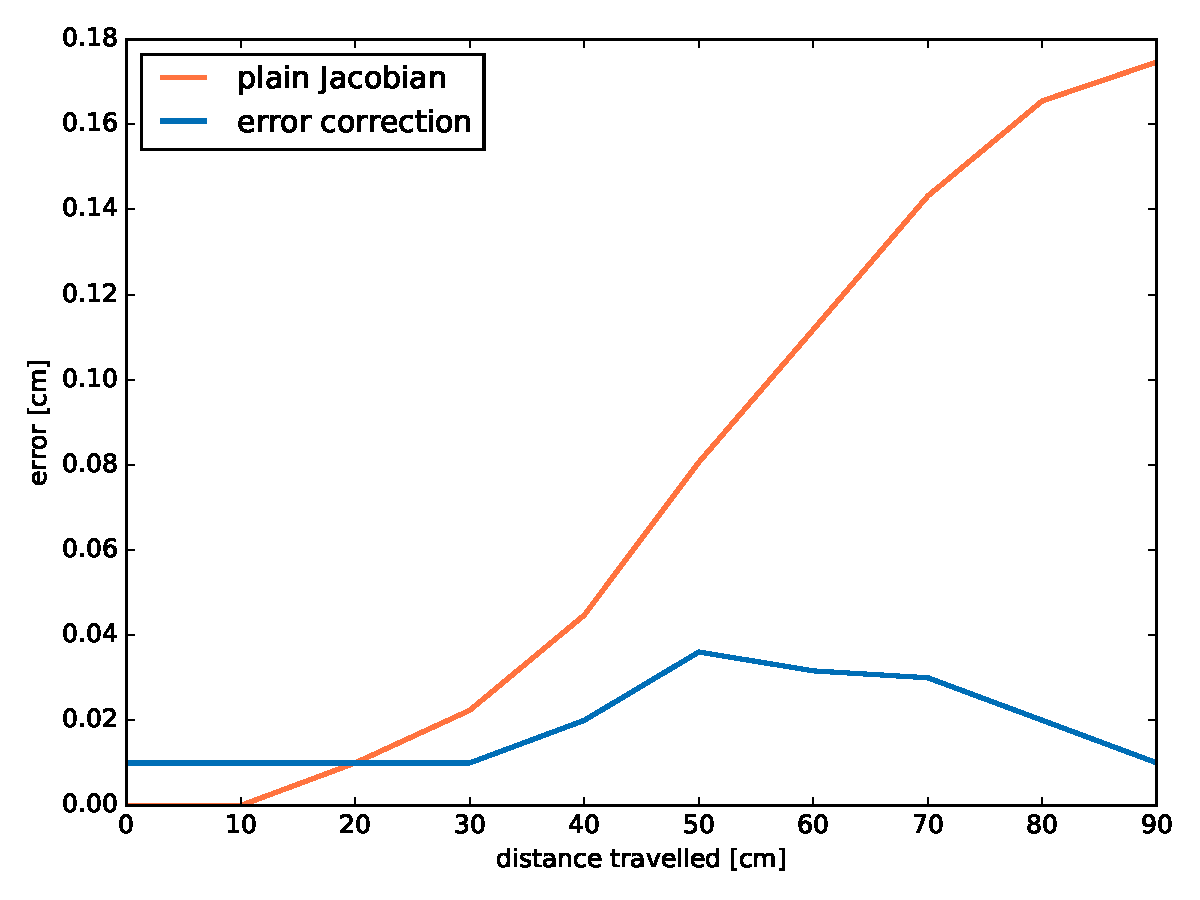
\includegraphics[width=7cm]{jacob_error_sim.pdf}
  \caption{Position error during simulated test drive}
  \label{fig:err_jac_sim}
\end{figure}

The error is probably caused by the numerical error attained in integrating the speeds in discrete steps in the control loop.

In some cases, mostly directly in front of the arm base, a near singularity is reached. Such configuration appears in the test trajectory at 45\,cm, where the end effector passed in front of the base. While we attempt to solve things by slowing the arm down (see the implentation details in Section~\ref{subsec:impl_drv_jacob}), in some configurations, we get so close to the exact singular configurations that no slow-down helps. The driving algorithm identifies such situations and reports failure to higher layers.

The final combined solution described in Section~\ref{subsec:impl_drv} proved to combine the best properties of both the methods. The fallback to planning is used exactly when neccessary. In some cases, however, the Jacobian motion gets the arm stuck in an unexplored collision box because of a slow collision check. Then, even planning fails to move to explore that cell and it is misclassified as unreachable. This results in false positive obstacles identified in the environment.

\subsection{Exploring 3D environment}
\label{subsec:sim_arm_cover}

We tested the final coverage algorithm first in the simulator. We ran it first in empty environment, then in the benchmark environment. The benchmark environment was simulated by publishing false force readings when the arm explored an occupied point.




\section{Real arm experiments}
\label{sec:exp_real_arm}

\subsection{Moving the arm}
\label{subsec:label}

We aimed to confirm the results of movement simulation on the real hardware. Motion planning exhibited the same bahavior as in the simulation. It worked reliably, but in some seemingly random cases, a very complicated plan was generated. These complicated motion plans threaten both the spectators and the cable linking the sensing tool to the host computer.

When we repeated the Jacobian control test we used with the simulated arm, we discovered that the real arm deviates from the intended trajectory significantly. After following the same trajectory, the arm deviated 6\,cm in \m y and 4\,cm in \m z direction. In the and, we had to cerrect the arm considerably in both location and orientation. We assume the error was given by our negelction of the arm dynamics, which we implement by assuming the given joint velocity can be reached immediately by the arm.

To compensate the error, we combined the velocity given by the exploration algorithm with a correction term, which keeps the arm on the defined line as described in . The results of the corrected control algorithm is significantly better, staying within 2\,cm of the line. The errors are depicted in Figure~\ref{fig:err_jac_real}.

\begin{figure}[ht]
  \centering
  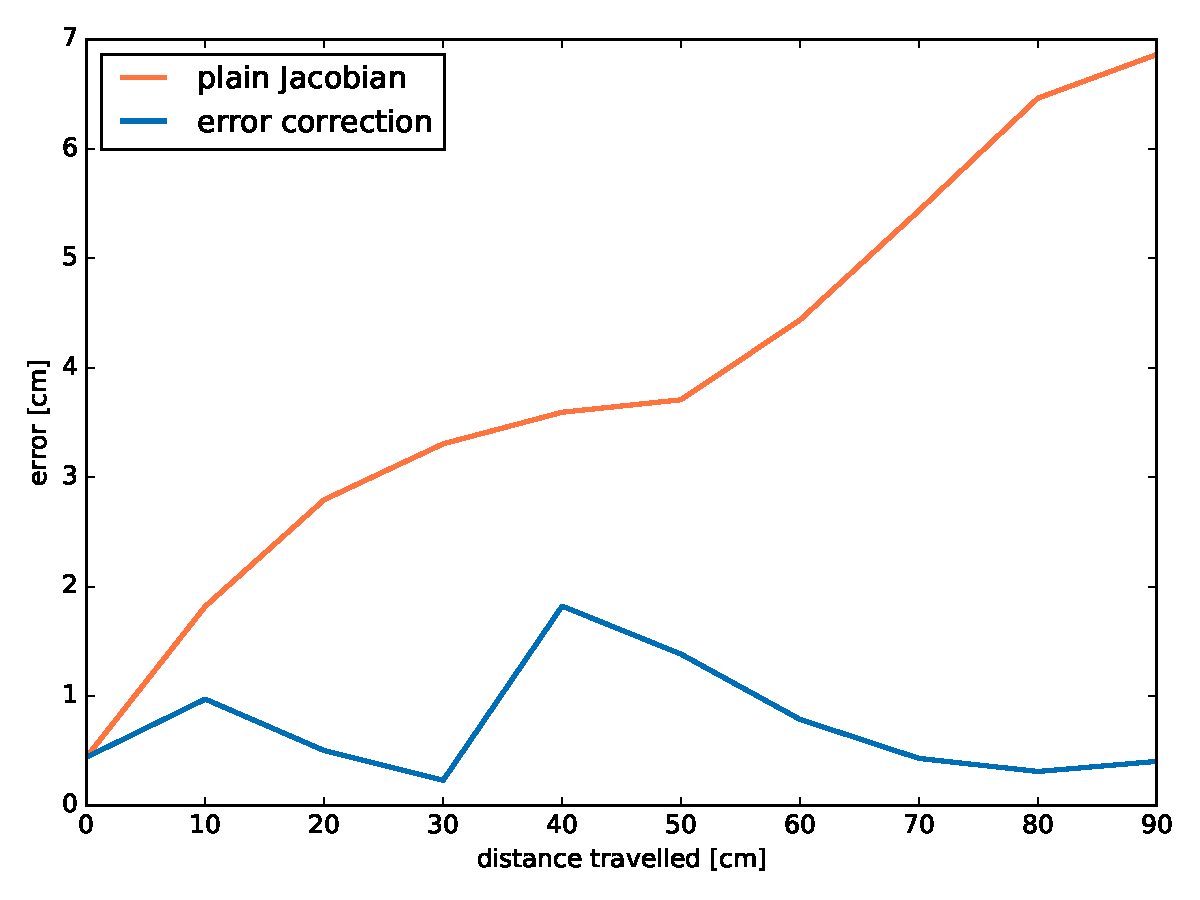
\includegraphics[width=8cm]{jacob_error_real.pdf}
  \caption{Plot of position error during the real test drive}
  \label{fig:err_jac_real}
\end{figure}

Another issue we noticed was that the movement was in no case as smooth as in the simulator. The arm came to a complete stop every time a decision was made on where to continue. The movement became nearly as jerky as the planned movement. We account this error to the arm dynamics as well, as getting the arm to move seems to take as much time as planning the next step. This could in the future be resolved by splitting the driving and planning into two independent computations, where the next direction would be known even before the arm arrives at the target position. We did not implement the solution due to its fearsome implementation complexity.

\subsection{Exploration of 3D space}
\label{subsec:label}



\end{document}


%%% Local Variables:
%%% mode: latex
%%% TeX-master: "buriama8_dp"
%%% End:
